\documentclass{article}
\usepackage{booktabs}
\usepackage{multirow}
\usepackage{caption}
\usepackage{float}
\usepackage{graphicx}

\begin{document}
\begin{figure}[H]
    \centering
    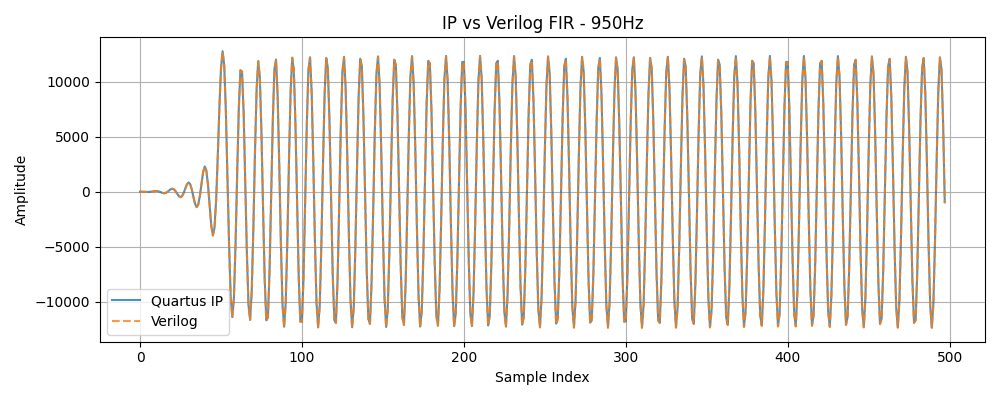
\includegraphics[width=1.0\textwidth]{Figure_950.png}
\end{figure}

\begin{figure}[H]
    \centering
    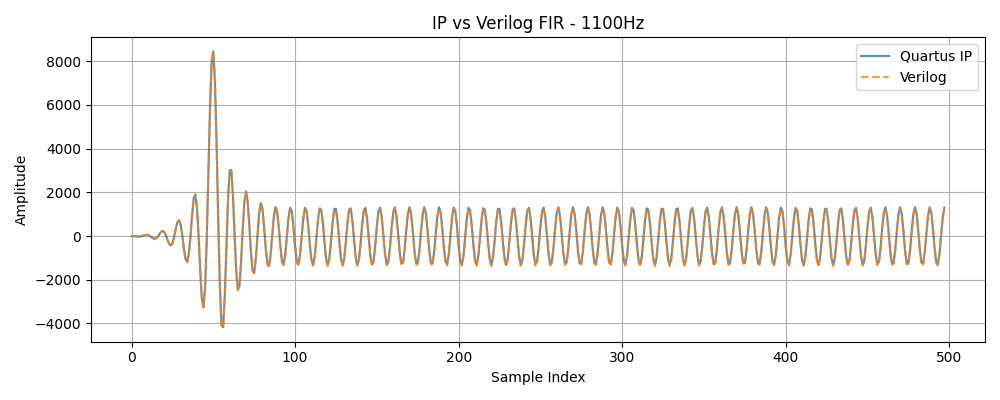
\includegraphics[width=1.0\textwidth]{Figure_1100.png}
\end{figure}

\begin{figure}[H]
    \centering
    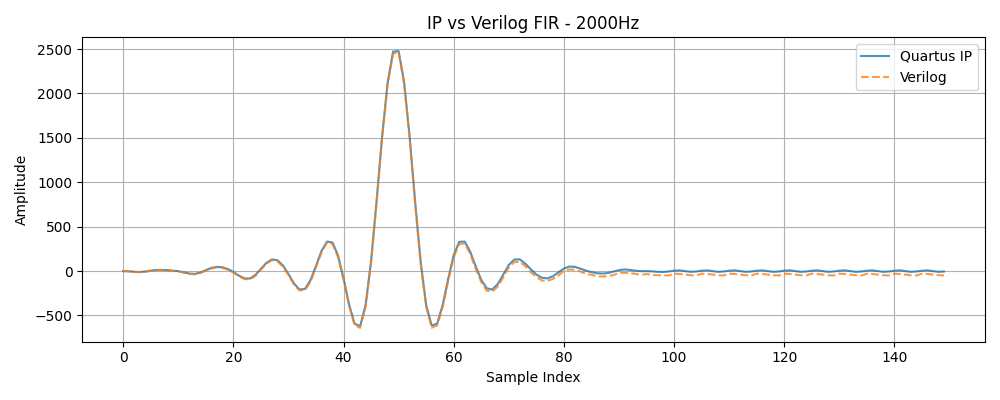
\includegraphics[width=1.0\textwidth]{Figure_2000.png}
\end{figure}


\begin{table}[htbp]
    \centering
    \caption{Performance and Resource Utilization Comparison}
    \vspace{0.2cm}
    \begin{tabular}{@{}lcccccc@{}}
        \toprule
        \multirow{2}{*}{\textbf{Architecture}} & \multirow{2}{*}{\textbf{$F_{max}$ (MHz)}} & \multirow{2}{*}{\textbf{Slack (ns)}} & \multirow{2}{*}{\textbf{Throughput (MS/s)}} & \multicolumn{3}{c}{\textbf{Resource Utilization}} \\ 
        \cmidrule(l){5-7}
        & & & & \textbf{ALMs} & \textbf{Regs} & \textbf{DSPs} \\
        \midrule
        Quartus IP & 180.18 & 3.07 & 180.18 & 1445 & 2863 & 25 \\
        \midrule
        \multicolumn{7}{@{}l}{\textit{Non-Pipelined Implementations}} \\
        Direct    & 44.86 & 2.707 & 44.86 & 1064 & 1727 & 25 \\
        Optimized & 46.82 & 3.76  & 46.82 & 1075 & 2727 & 25 \\
        Genvar    & 51.86 & 5.704 & 51.86 & 4099 & 1872 & 0 (logic) \\
        \midrule
        \multicolumn{7}{@{}l}{\textit{Pipelined Implementations}} \\
        Direct    & 191.02 & 19.198 & 191.02 & 1075 & 2785 & 25 \\
        Optimized & 195.82 & 19.765 & 195.82 & 1572 & 2785 & 25 \\
        Genvar    & 221.04 & 20.476 & 221.04 & 1572 & 3173 & 25 \\
        \bottomrule
    \end{tabular}
    \label{tab:performance_comparison}
\end{table}

\end{document}
